\chapter{Problem Formulation}
\label{sec:relevant-knowledge}
The translational dynamics of the chaser are considered to be in the local-vertical-local-horizontal (LVLH) frame of reference of the target.
As depicted in Figure \ref{fig:lvlh_frame}, this reference frame is centered at the center of mass of the target and fixed with respect to the orbit with its Y-axis pointing radially into the center of the Earth, the X-axis pointing opposite to the direction of the velocity of the target spacecraft, and the Z axis pointing along the angular momentum vector of the target, hence completing a right-handed system.
\begin{figure}[htb]
    \centering
    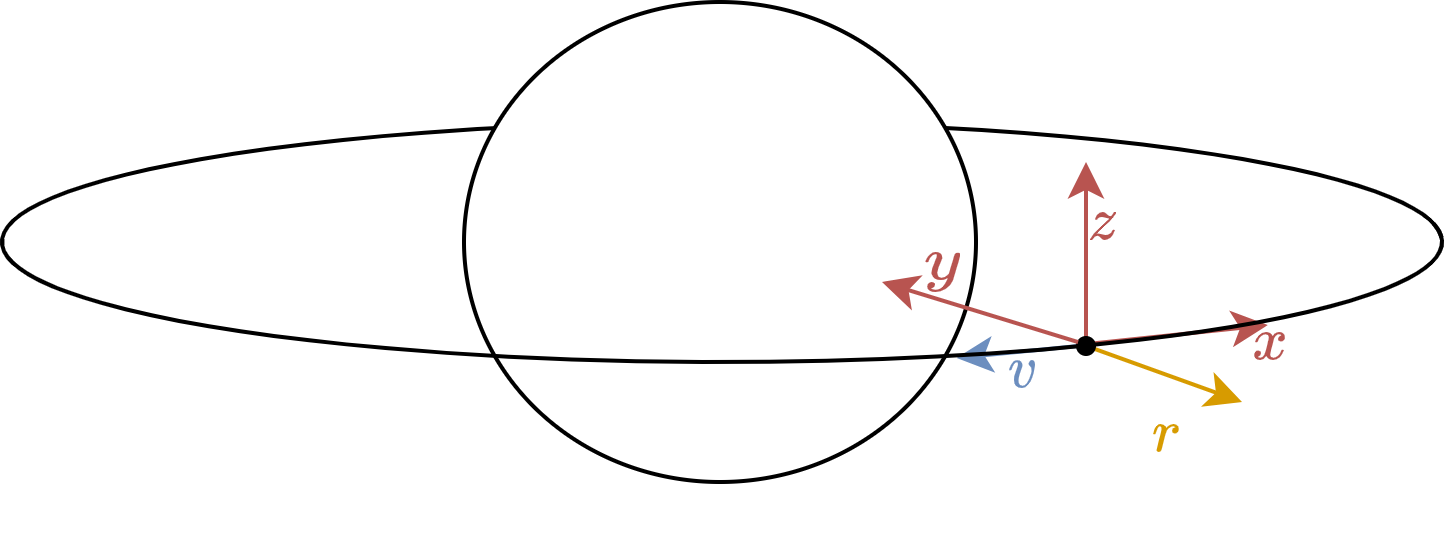
\includegraphics[width=0.9\linewidth]{assets/lvlh_frame.png}
    \caption{Local-Vertical-Local-Horizontal Frame of Reference of the Target.}
    \label{fig:lvlh_frame}
\end{figure}
If we assume the orbits of the target and the chaser to be circular, within close proximity to the target, the translational dynamics of the chaser follow the Clohessy-Wiltshire-Hill (CWH) equations (refer to Appendix \ref{app:cwh-equations}).
However, in this paper, we generalize the problem to targets that may be in elliptical orbits around the Earth.
Appendix \ref{app:ellp-undrag} describes the dynamics of relative motion in an elliptical orbit where the chaser and the target may have unequal drag constants.
These dynamics apply to the chaser with respect to the LVLH frame of reference (refer to frame L in Figure \ref{fig:target-cylinder}).
As considered in \cite{carter2002clohessy}, we assume an inverse law, $g(R)=1/R$, to model the variation in atmospheric density.
However, we realize that this inverse law does not perfectly represent the scale of the trend of atmospheric density \cite{emmert2021nrlmsis}.
As a result, we consider the corresponding ratio in variation into the drag constants $\alpha$ and $\beta$ of the target and the chaser respectively.
Such a system considers the true anomaly $\theta$ of the orbit as the independent variable, hence giving the following dynamical equations:
\begin{align}
    \boldsymbol{r}'(\theta)&=A(\theta,\theta_0)\boldsymbol{r}(\theta)+B\boldsymbol{u}(\theta)+\boldsymbol{d}(\theta, \theta_0),\label{eqn:dynamics}
\end{align}
where
\begin{subequations}
\begin{align}
    \boldsymbol{r}(\theta)&=\begin{bmatrix}
    x(\theta),y(\theta),z(\theta),x'(\theta),y'(\theta),z'(\theta)
    \end{bmatrix}^T,\\
    \boldsymbol{u}(\theta)&=\begin{bmatrix}
    u_x(\theta),u_y(\theta),u_z(\theta)
    \end{bmatrix}^T.
\end{align}
\end{subequations}
We will consider true anomaly to be the primary independent variable throughout this paper so it will be omitted as the state and input variables argument for clarity.
The relation between the true anomaly of the target and the time lapsed $t=t_{\text{curr}}-t_p$ since periapsis (the point in the path of the chaser-target system at which it is nearest to the Earth) is given as:
\begin{subequations}
\begin{align}
    M&=M_0+2\pi\frac{t}{T},\\
    M&=E-{\mathsf{e}}\sin(E),\\
    \theta&=E+2\arctan\left(\frac{\beta\sin(E)}{1-\beta\cos(E)}\right),
\end{align}
\end{subequations}
where
\begin{equation}
    \beta=\frac{{\mathsf{e}}}{1+\sqrt{1-{\mathsf{e}}^2}},
\end{equation}
$M$ is the mean anomaly of the target, $E$ is the eccentric anomaly of the target, and ${\mathsf{e}}$ is the eccentricity of the orbit of the target.
Hence, the true anomaly of the orbit can be numerically computed from time and time can be analytically computed from true anomaly.
\begin{figure}[htb]
    \centering
    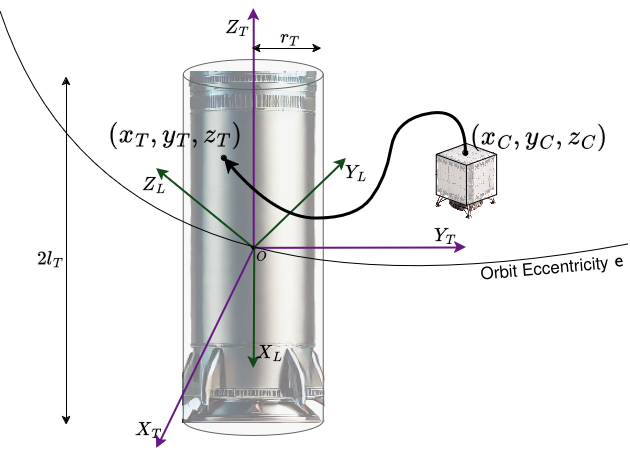
\includegraphics[width=0.85\linewidth]{assets/target-cylinder.png}
    \caption{Frames of Reference centered at the Target. The axes with subscript $T$ belong to the body frame of the target that rotates with the target and the axes with subscript $L$ belong to the local-vertical-local-horizontal (LVLH) frame that is defined in Chapter \ref{sec:relevant-knowledge}.}
    \label{fig:target-cylinder}
\end{figure}

% To follow consistent nomenclature, we use \theta in this paper to represent the true anomaly of the chaser-target system and \boldsymbol{\theta}\boldsymbol{\theta} to represent the angular position of the target.\\
\section{Summary}
This chapter presents information relevant to the setup of the problem statement.
This involves the orbital dynamics of the chaser in the frame of reference that is under consideration - the local-vertical-local-horizontal (LVLH) frame of reference.
While the Clohessy-Wiltshire-Hill equations (with time as the independent variable) are used in a circular orbit, we propose the use of the Tshauner-Henkel equations that are subsequently modified to incorporate atmospheric drag. 
These equations define the dynamics of the chaser in an elliptical orbit and use the true anomaly of the orbit as the independent variable.
As a result, the chapter also provides insight into the relation between time since periapsis and the true anomaly of the orbit through the mean anomaly and the eccentric anomaly.